\chapter{Developed Peer-to-Peer Communication Prototype}
\label{chapter:work}

In this chapter the implementation of the developed peer-to-peer communication prototype will be analysed. This explanation will extend from the decisions of the technology and protocols to use to the architecture and workflow of the application.

It will begin with a brief summary of the steps taken to reach the developed application's features, functionalities and architecture. Which obstacles led to this solution and which were the fundamental drivers to decide upon this development and architecture to solve the problems previously stated. After the overall application's objectives and high-level architecture is described, a section on the lower-level architecture and components of the application will be presented, also containing flowcharts and diagrams on its normal functioning. A summary on the limitations and future work of this application will be given, as well as some possible solutions to its current limitations, outside the scope of this work. Finally, a conclusion on the difficulties and drawbacks of the development process and overall project appreciation will be given, along with some final thoughts on the work process and methods used.

\section{Peer-to-Peer Application Design Choices}

This section will provide the explanation and justification of the choices made for the application traffic type, ad hoc communication technology and ad hoc routing protocol.

In section \ref{sec:wfd}, developed work on Android applications using Wi-Fi Direct has a mean of communication was introduced. Having the guidelines of these works in mind, the development of this application started. The main structure would always be: the application will have a routing algorithm that controls the destinations of the packets in each hop. A communication technology, \textit{e.g.} Bluetooth or Wi-Fi Direct, handler for both discovering nearby devices and establishing communication sockets with peers. A set of functions capable of analyzing incoming messages and deciding which is the next step to perform, in order to complete the requests/advertises. Finally, a user interface where the incoming messages can be seen and analysed (for debug purposes), also providing a text area for the user to enter the requested data.

\subsection{Application Traffic Type}

The choosing of what would be the transferred data between devices was one of the major steps of this work. Many ideas could be pursued and each one of them could be a great work to develop. The main contenders were text messages, beacon messages, geolocation messages and web pages. After some research was made, see section \ref{sec:apps}, some of these contender could be eliminated, due to the existence of works already revolving around them. The main topic was text messages with many of the works developed focusing on recreating popular applications, such as Messenger and WhatsApp, using a peer-to-peer network to route the messages to their destinations. Beacon and geolocation messages were also not a completely innovative choice, since applications such as Uepaa!, see subsection \ref{subsec:uepaa}, are already implementing systems similar to the one being proposed. Given this reasoning, the most innovative choice would be to transfer web pages between devices, creating a multi-hop hot spot in a peer-to-peer network.

\subsection{Ad Hoc Communication Technology}

After being established that web pages were the data to be requested, the next step was to choose the communication technology to be used, followed by the routing algorithm that would manage the next hops to take. The first and most obvious choice would be to use Wi-Fi Direct in both advertising and communication between devices, since this technology offers the best features to transfer files around 1Kbyte, in both range and data rate of transmission. However, during the development it proved to be impossible to continue with this approach, as Wi-Fi Direct's current Android implementation does not allow for devices to transfer files without user consent.

Given this drawback a shift to Bluetooth was made, and a hybrid version of the application was created, where the advertisement would be done via Wi-Fi Direct and the actual transfer of the web pages would be made via Bluetooth. This method also proved to be infeasible, due to security issues, since the the devices would have to display their Bluetooth MAC addresses in their Bluetooth name, making them much more vulnerable to possible attacks.

So, finally, the application was developed using Bluetooth for both advertisement of the devices and data transfer, although this is not the best technology for communication in a peer-to-peer network, it is the only one that, currently, meets all the requirements for this work. In the end of this chapter a brief discussion on the changes that need to be made to Wi-Fi Direct's implementation in Android will be presented, and why developers could benefit from these changes.

\subsection{Ad Hoc Routing Protocol}

The last step would be to create/modify a routing algorithm to control the destination of each incoming message. The requirements are simple, the algorithm simply needs to save the next hop of the shortest path leading to a device with Internet connection.

\gls{AODV} is a known routing scheme used in ad hoc mobile networks, precisely what this application will establish with the devices. However, it establishes dynamic paths, \textit{i.e.} only when a device wants to retrieve a web page does this protocol searches for a path in which to send the packet, see \cite{aodv} for the full specification of this scheme. This scheme is not the best for the applications reliability, since the requesting device should know before hand if it is capable of reaching the Internet, otherwise users will experience long periods of path requesting and advertising every time they request a web page.

\gls{DSDV} is also known for its use in ad hoc mobile networks. This protocol uses a routing table where it stores in each entry: the destination, next hop, number of hops to reach the destination and a sequence number - avoiding routing loops. The devices exchange full routing tables, creating a network where every device has total knowledge of the topology, being a powerful advantage. However, \gls{DSDV} requires the exchange of routing tables and their regular updates, using unnecessary bandwidth, see \cite{dsdv} for more information on \gls{DSDV}.

Since the routing of this work does not have a specific destination as a goal, in other words, device A does not want to transmit to B, it only wants to reach a node with network access with the minimum amount of hops, so A does not have knowledge on where its message will be sent after the immediate next hop. Thus, in order to accommodate such requirements some modifications were made to \gls{DSDV}. Firstly, to reduce the bandwidth used by \gls{DSDV}, this adaptation will simply exchange the best estimate of the current device, only including the number of hops and the device's \gls{MAC} address. Secondly, instead of a periodic exchange of tables, devices will update their tables every time a new advertise message is received and they only exchange routing information when a new best path is received, with the contents described above.

\section{Architecture}
\label{sec:architecture}

In this section the architectures of both framework and application are presented. It will consist of: a description of the Bluetooth connections between devices, an explanation on the discovery and advertising mechanism and a analysis of the web page exchange process.

\subsection{Bluetooth Connections}
\label{subsec:btconn}

In this subsection the Bluetooth connections between devices and their possible stages will be described and analysed.

Since the communication technology is Bluetooth, the application must have a thread\footnote{Thread is a sequence of instructions managed independently, usually by a scheduler from the operating system, see \cite{threads} for more documentation on threads.} that handles the listening and acceptance of connections and the data transfer between devices. This corresponds to the \textit{BluetoothService.java} class, from the application. It creates and listens to insecure communication sockets allowing devices to exchange data without user approval.

The service has three different threads within it: a thread for the acceptance of incoming communications - \textit{AcceptThread}, a thread for the initial exchange of vital information before the connection - \textit{ConnectThread} - and a thread for the actual exchange of data between devices - \textit{ConnectedThread}. The connection of devices goes through each of these stages, allowing the main thread to get information on what is the connection status of the device at a given time.

There were two different approaches to the connections of devices: either the devices stayed connected as long as possible until a new connection was requested or the devices stayed connected for the minimal amount of time for data to be transferred. The second approach was used, since it is the one that is more energy efficient, draining a lower amount of battery from the devices.

Bluetooth communication between devices is only allowed if both devices have matching "credentials", providing a minimum amount of security to prevent against possible attacks. An application specific name and \gls{UUID} represent the application, making it distinguishable from any other, since the \gls{UUID} of an application should not be repeated in any other.

To notify the application of what is being done by the \textit{BluetoothService} a handler is created, acting as bridge between the two parts. It can be used for various actions, such as: retrieving the status of a connection, assessing if a device is ready to receive a file, \textit{etc.}

To substantiate the possible Bluetooth connections stages four different textual representations are created, one for each stage: listening, connecting, connected and not enabled. Each type of thread mentioned earlier is associated with one stage, being the non-existence of a thread the not enabled stage. The different threads can be seen as the implementation of a stage. They are the ones that dictate how is the application going to act during the stage. 

In the next subsections each stage will be explained in detail, providing a better understanding on how the connections are performed.

\subsubsection{Listening}
\label{subsubsec:listening}

A device is said to be in the listening stage when it has no ongoing connection but it is waiting for a new one initiated by another device. It is the "first" stage of the \textit{BluetoothService}, since every time the service is initiated the device is moved to this stage.

As was said previously, each connection stage is associated with a thread class. The listening stage is associated with the \textit{AcceptThread}, which is instantiated every time the device enters this stage. The framework's connections have short durations and each time a new connection is performed the service is restarted, entering the listening stage. Hence, it is imperative to assure there are no memory leaks or communication sockets left open. Thus, before the listening thread is instantiated it is verified if any other Bluetooth connection threads are running and, if so, they are shut down.

Once all the requirements for the instantiation of a new thread are met, a communication socket is created with which the device listens to incoming communications. To implement the listening mechanism a loop is created whose purpose is to block the thread until a new connection is received, an error occurs or the user shuts down the application.

Whenever the device receives a new connection, it verifies the "credentials" sent in that request and compares them with the ones defined in its application. If they match the connection is accepted.

Upon successfully accepting a connection, the method assesses the status of the newly formed connection and decides upon it. If everything goes as planned, the connection should now be in the connected stage. Once this migration between stages is concluded the instance of the listening thread is destroyed, for reasons above stated and the 

\subsubsection{Connecting}
\label{subsubsec:connecting}

Concluded the listening and accepting of connections it is necessary to understand how they are requested. For a Bluetooth connection to be performed at least two devices must exist, one of them acting as the connection requester.

Similar to the listening thread initiation, the \textit{ConnectThread} is only instantiated after all the previous Bluetooth connection threads running in the device are shut down. Also, to avoid delays during the connection process, the Bluetooth discovery process is shut down. Only then can the requester attempt to establish a connection with the desired device.

To identify the receiver of the connection request, the device needs to retrieve the \gls{MAC} address of its counterpart, this will be explained in subsection \ref{subsec:disandadv}. Once this is attained the requester can attempt to create a communication socket between both devices, using the previously defined Bluetooth "credentials" and the receiver's \gls{MAC} address. If the \gls{MAC} address is valid and corresponds to a device within reach the connection is request successfully.

In case of failure due to the rejection of the connection from the receiver, a notification is sent to the application, notifying the connection was not successful and the service is restarted.

However, if the sent request is accepted by the receiver, the connection state is assessed and, if no interruptions or errors occur, the connection stage is moved to the connected stage, indicating both devices are able to send and receive bytes from their counterpart, by writing and reading from the established communication socket, respectively.

\subsubsection{Connected}
\label{subsubsec:connected}

The \textit{connected()} method is called in both requested and requester devices, it is called upon concluding the preliminary works of the connection. It starts by canceling any ongoing threads, again in order to avoid conflicts between the device's Bluetooth communications. It then creates an instance of the \textit{ConnectedThread} and sends back to the main activity the name of the device with which the connection was just established. Finally, it sets the communication status to \textit{STATE\_CONNECTED}.

The \textit{ConnectedThread} class follows the same pattern as the other two thread classes. It has a constructor but it has four methods: the constructor receives the established communication socket and creates an \textit{InputStream}\footnote{An InputStream is an abstract object created to read bytes from a source of data, see \cite{inputStream} for full documentation.} and \textit{OutputStream}\footnote{An OutputStream is an abstract object created to writes bytes to a source, \textit{e.g.}, a file or a socket, see \cite{outputStream} for full documentation.}, in order to read and write bytes to the socket shared with the other device, respectively. The \textit{run()} method has a cycle that keeps reading from the socket to a buffer while the connection is not closed. Since we send two different types of data from device to device, strings and web pages, logic was created in order to distinguish what is the device expected to receive at any given time. The variable \textit{fileReady}, as mentioned previously, is used to assess if the device is ready for the reception of a web page, by checking the status of this variable the application infers if it should treat the received data as a string or a file. Should the variable return false, meaning the device is not ready for file reception, the service will send the received string to the main activity, via the handler, so that the message can be analysed and the next step can be decided, otherwise, the device is ready to receive the web page. In order to overcome the size limitation of the socket buffer, approximately 1Kb, the web pages are disassembled in smaller chunks of 990 bytes. A auxiliary buffer is created to store the received chunks, orderly, and, by judging the size of the chunks, the receiver can assess if it is receiving the last chunk, \textit{i.e.}, by comparing the received number of bytes and 990. After the reassembly of the chunks is done, the bytes are sent to the main activity to be processed. In case the connection is suddenly broken, the \textit{connectionLost()} method is called, notifying the main activity of this event and restarting the service.

The next two methods, \textit{write()} and \textit{writeFile()} are called by the sender device to write bytes to the \textit{OutputStream}. It is important to make the differentiation between writing a simple string and a file because of the above mentioned disassemble and reassemble of the file chunks, which is not necessary when working with strings. So if the message to send is a string, containing information on an advertise, request, response or failure, it will be handled by the \textit{write()} method, simply writing the bytes to the socket and notifying the main activity of that action. However, if the data to be sent is a file, it will have to be divided into chunks of 990 bytes as mentioned before, also, since the service needs to notify the stream on the exact amount of bytes to be transferred, extra logic is needed to get the number of bytes that the last chunk of the file contains. Both these methods can be called asynchronously, \textit{i.e.}, by user request, via two functions of the service, \textit{write()} and \textit{writeFile()}, whose functionality is simply to call the \textit{ConnectedThread} class's functions, respectively.

Finally, the \textit{cancel()} method serves a similar purpose to the previous classes, it forces the close of the socket and nullifies the thread instance.

\subsection{Discovery and Advertising}
\label{subsec:disandadv}

Now that the basic concepts on how the communication between devices are implemented are explained, it is possible to dig deeper into the intrinsics of the application itself, and what is the logic behind the routing of web pages.

The first thing in order for each device to know what is the next hop of a certain request will be to fill the routing tables. This process is done by a series of discoveries\footnote{Discovery is the act of finding nearby devices with Bluetooth on.} and advertises\footnote{Advertise is the act of notifying peer devices of the cost of relaying a request to the device issuing the advertisement.}. Upon starting the main activity each device will advertise its best estimate to reach the Internet. This advertise will be received by peers and analysed, in case the estimate of relaying the requests through that node improves the current estimate, the receiving peer will begin another discovery and advertising process with the newly discovered path. Otherwise, the peer will add or update an entry in the routing table, regarding the advertiser.

\begin{figure}[ht]
   \noindent\makebox[\textwidth]
    {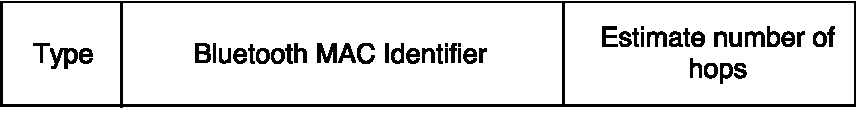
\includegraphics[width=0.7\textwidth]{images/adv_message.pdf}}
	\caption{\label{fig:advmsg} Advertising message format}
\end{figure}

In figure \ref{fig:advmsg} the format of an advertise message is shown. The type is a feature to common all messages exchanged in this application, it servers the purpose of identifying which type of message is being received. It can take four different values: \textit{ADV}, \textit{RQT}, \textit{RSP} and \textit{FAIL} for an advertise, request, response and fail message, respectively, in this case it will take the value \textit{ADV}. The delimiters of the different message parts - vertical lines in the figure - are represented by the dot comma character (;), in order to be able to separate the different parts of the message. The Bluetooth \gls{MAC} identifier is always the \gls{MAC} address of the Bluetooth adapter of the sender, it is then used by the receiver to populate its routing table. Finally, the estimate number of hops is the smallest number of hops the sender needs to be able to reach the Internet plus one, corresponding to the hop from the receiver to the sender.

Each device has two different routing tables: one that is accountable for routing the requests to the final device and another one that is accountable for routing the responses to the original sender and it will be analysed in the next subsection. For simplicity the first routing table will remain with this name, while the second will be referred to as response table, as it handles the routing of responses.

\begin{table}[ht]
\centering
\bgroup
\def\arraystretch{2.5}
\begin{tabular}{|c|c|}
\hline
\textbf{Next hop's MAC} & \textbf{Number of hops} \\ \hline
Own MAC & 0 or 16 \\ \hline
Device A's MAC & Estimate through A \\ \hline
Device B's MAC & Estimate through B \\ \hline
... & ... \\ \hline
Device Z's MAC & Estimate through Z \\ \hline
\end{tabular}
\egroup
\caption{Routing table example and format}
\label{tab:routTables}
\end{table}

In table \ref{tab:routTables}, an example of a routing table is presented, where the first entry is always populated with the device's own \gls{MAC} address and its estimate, which is either 0 or 16\footnote{16 was chosen to be the representation of infinity or inability to reach a destination, since it has been represented by this number in various protocols, for instance in \gls{RIP}, see \cite{ripprotocol}}, meaning the device has an Internet connection or not, respectively. Every time a device receives an advertise message, it populates this table, either by adding a new row or updating an existing one, with the information contained in the message, see figure \ref{fig:advmsg}. When the routing table is done being populated, each node knows its immediate peers and the best estimate through each peer, giving it a full knowledge on its vicinity, not on the overall network.

In the code, this process was implemented, mainly, in \textit{RoutingApp.java} class and in the main activity, or \textit{BtActivity.java}. Let's start by understanding how the routing tables are being created and, posteriorly, it will be explained how and when they are populated. It is important to note that \textit{RoutingApp} class extends the Java class \textit{Application}, meaning that, with the exception of the private methods and variables, every part of this code can be accessed at any time in the application, in contrast with other activities that are only accessible when active, such as \textit{BtActivity} and \textit{InitActivity}.

In appendix \ref{appendix:RoutingApp} it is possible to see the definition of two tables \textit{routeTable} and \textit{rspTable}, corresponding to the routing table and response table, respectively. In this subsection's scope a closer look will be taken on the first table. It is represented as an instance of the Java interface Map\footnote{In Java, a Map is an object that relates keys to values. To a single key corresponds a single value, thus not creating duplicate entries, see \cite{map} for full documentation.} where the keys correspond to the \gls{MAC} address of the next hop, the string, and the keys to the respective estimated number of hops, the integer. So it maps a string to an integer, which is the same to say that given a string the table contains, it will return an integer.

There are three important features that the application needs from this table: to get the absolute minimum value, meaning retrieving the lowest possible value for any given key, in order to retrieve the device's best path. To get the corresponding key to the minimum value, in order to retrieve the receiver to whom this device should send the message. Finally, to update or add a row with a new key-value pair, in order to add newly received advertising information.

The first feature is completed by method \textit{getMinHop()}. This function starts by creating a variable \textit{minHop}, that will be assigned to the minimum value of the table. It then makes use of the preexisting Java method \textit{Collections.min()}, that returns the minimum value from a set of values, and assigns the variable \textit{minHop} to this value. To get the desired value, it is given the set of values of the routing table, by calling \textit{routeTable.values()}. Should this succeed, the function will return the desired value, otherwise it will return 16, for the reasons explained above.

Having the minimum value from the routing table, it is now necessary to retrieve the \gls{MAC} address from the device that provides this estimate. This is done by function \textit{getKeyFromValue()}, that receives the routing table itself and the desired value. It iterates through every key and, in every iteration, it compares the value of the current key to the expected value, since it already knows the minimum value it is useless to compare the values of the different keys. If, in a given iteration, it finds a key that maps to the desired value, this key will be returning, corresponding to \gls{MAC} address of a device that gives the smaller estimated number of hops, otherwise it returns null. It is important to note that several devices may provide the shortest path, but the application will only chose the one that was found first, since they all provide the same estimate.

Finally, the addition and update of rows within the table is done by the method \textit{updateRouteTable()}, that takes as arguments the newly received advertising message. It begins by fragmenting the message in its parts, knowing that, according to figure \ref{fig:advmsg}, this message will contain the type in the first position\footnote{In Java, the first position of an array is given by the number 0, the second by the number 1 and so forth, see \cite{arrays} for more information.}, the sender's \gls{MAC} address in the second position and the estimated number of hops in the third, using dot commas as delimiters. Using Java method \textit{String.split()}, the function separates the string by dot commas, creating an array of smaller strings, it then matches the destination to the second position, represented by variable \textit{dest}, and the number of hops to the third position, represented by variable \textit{hops}. Having this information, the Java method \textit{Map.put()} is used, it inserts the given key-value pair into the existing table, in case this key already maps to a value, the value will be overwritten with the new one, otherwise it will simply insert the new pair as a new row, see \cite{map} for full documentation on this method. 

Note that, in case of a table update, the application does not compare values, \textit{i.e.}, it does not check if the new estimate is better than the old one, since the sender device could have lost the communication with the best route and thus it needs to advertise a worse path. If this check was made, the receiver could be mislead into sending requests through this device, thinking it would provide the better path.

\subsubsection{Discovering Peers}
\label{subsubsec:disc}

Now that it is clear how the intern process of modifying the routing tables works, it is possible to discuss where and when these methods are being called. Shifting the focus to \textit{BtActivity.java}, in appendix \ref{appendix:BtActivity}, there are some variable definitions indispensable for the process of advertising and discovery. Starting by the \textit{peers} \textit{ArrayList}, it is a list of \textit{BluetoothDevices} each corresponding to a peer found in the discovery process. This list is then used to retrieve information from these devices, in order to successfully establish communication sockets with them. The \textit{mBluetoothAdapter} is no more than the device's Bluetooth adapter, without which there would be no Bluetooth communications. Finally, the variable \textit{discoveryFinished} is a boolean value that serves the purpose of identifying if the discovery process is finished, assuring that this is not carried away for longer than it was intended to be, using processing power and damaging the performance of the rest of the application.

Method \textit{onStart()} is used to denote the starting of the activity. It  starts by verifying the necessary steps to ensure Bluetooth is properly set. Some configurations relative to an \textit{WebView} object, that will be discussed later, are performed. The \textit{ensureDiscoverable()} method is called, in which the application checks the Bluetooth visibility of this and, in case it is not discoverable, it sets the visibility to 0, that corresponds to "always visible", see \cite{btandroid}.

Once the Bluetooth is set up, the initial update of the routing table is performed, a quick network check indicates if the device has an active Internet connection, by calling the method \textit{getHasNet()}, from \textit{RoutingApp.java} class, in appendix \ref{appendix:RoutingApp}. Should the device return positive, it will add a new row with its own \gls{MAC} address, retrieved by method \textit{getOwnMAC()} and 0 hops, since it's connection is immediate. In case the Internet check returns negative, meaning the device is currently unable to reach it, the same process is performed, however instead of 0 hops, the estimate will be of 16 hops, for reasons already explained.

The device is now finished with the first steps of assessing its position in the network and filling its routing table accordingly. After this logic is accomplished the function \textit{doDiscovery()} is called, it sets the variable \textit{discoveryFinished} to false, indicating the discovery is not yet finished and commands the Bluetooth adapter of the device to initiate the discovery process.

Figure \ref{fig:adveg1} demonstrates how two devices, one without an Internet connection (left) and one with an active Internet connection (right). At this point both devices should have exactly one entry at their routing tables, since they have not communicated with any other device but they have established their position in the network, \textit{i.e.}, if they have an Internet connection. Device A is unable to reach the Internet, so it adds to the routing table an entry with its own \gls{MAC} address and an estimate of 16 hops. Device B, on the other hand, is able to reach the Internet, thus having an entry with its own \gls{MAC} address and an estimate of 0 hops.

\begin{figure}[ht]
   \noindent\makebox[\textwidth]
    {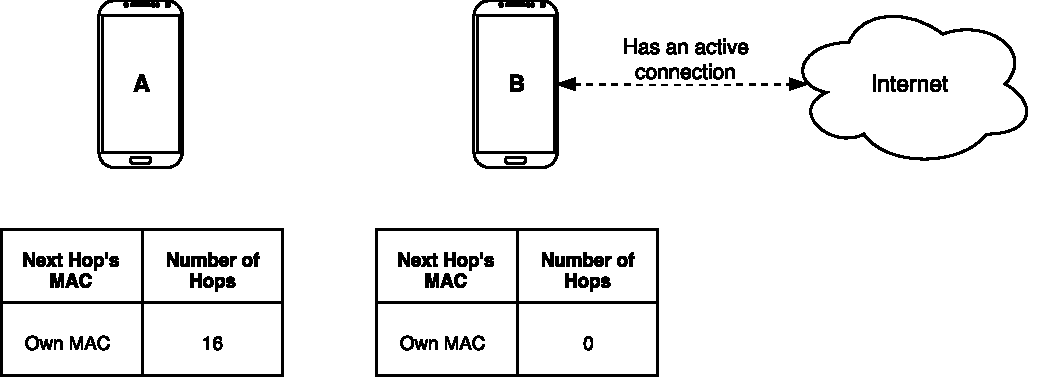
\includegraphics[width=0.9\textwidth]{images/adv_example_1.pdf}}
	\caption{\label{fig:adveg1} Example 1: State of the two devices after the initial step is over}
\end{figure}

Jumping now to the definition of the \textit{BroadcastReceiver mReceiver}, responsible for the management of the Bluetooth discovery process and peers found, we can see that it is divided into two main sections: one for the management of a peer found and other for the management of the finished discovery. In the first segment, whenever a device is found, a new \textit{BluetoothDevice} object is created, to designate the found peer, this peers is the added to the list \textit{peers}, unless this device is already part of this list. In the second segment, corresponding to the finish of the discovery process, the receiver checks if the variable \textit{discoveryFinished} has been toggled on, meaning it's the first time the device has received an \textit{ACTION\_DISCOVERY\_FINISHED} action, which is self-explanatory, so the discovery should be canceled, by \textit{cancelDiscovery()} and the variable \textit{discoveryFinished} needs to be set to true.

In figure \ref{fig:discflux} a fluxogram of the discovery process is presented. By following the figure it is possible to understand the flow of the code and the hierarchy of instructions. It is a visual representation of the code running. Note that it ends with the instruction \textit{advertisePeers()} that will be explained shortly.

\begin{figure}[ht]
   \noindent\makebox[\textwidth]
    {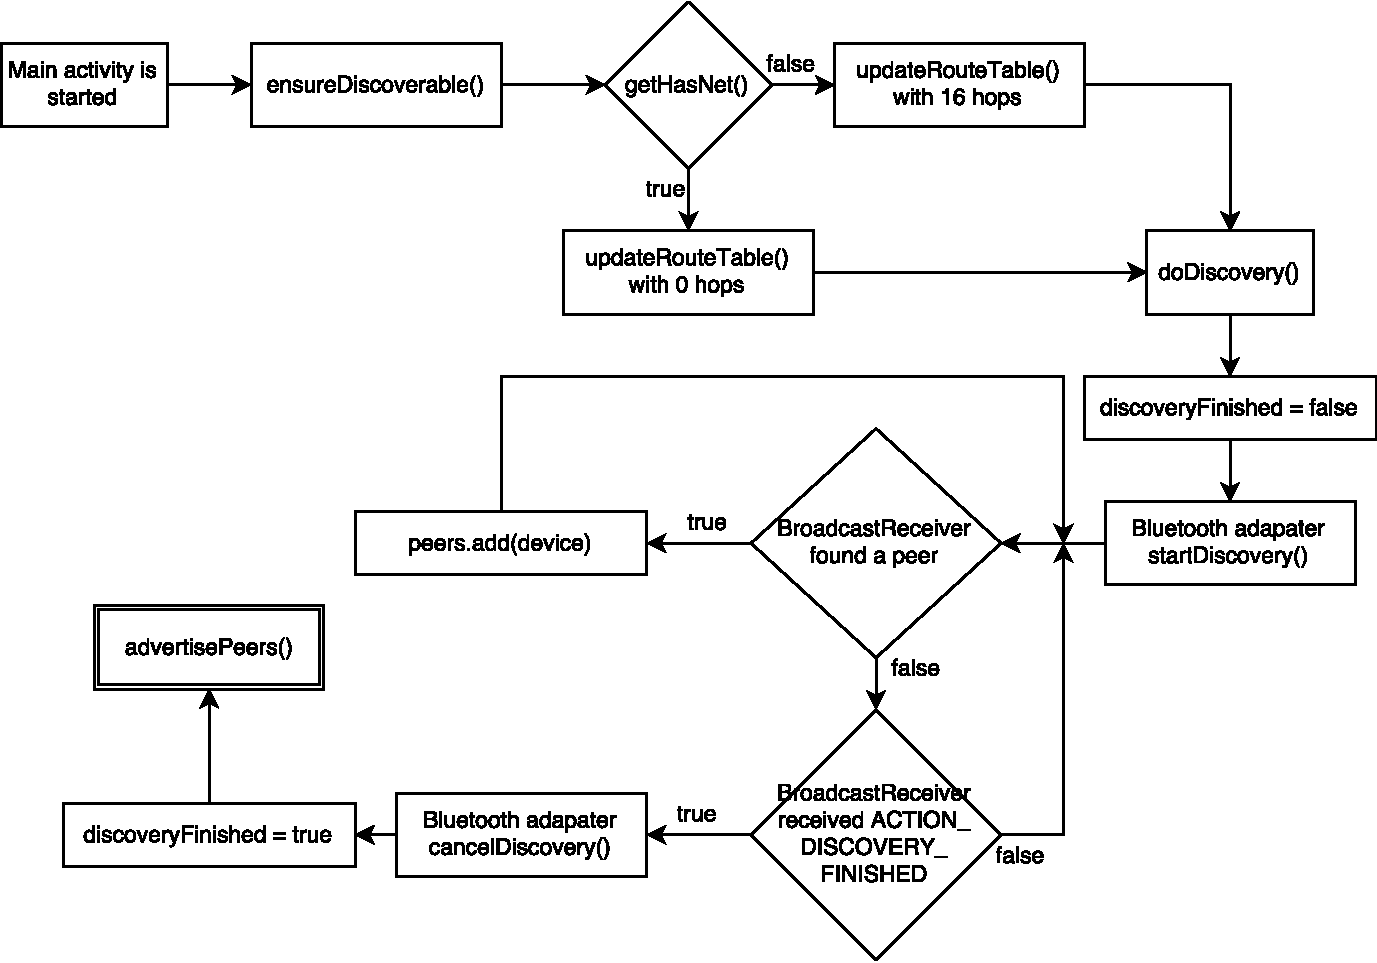
\includegraphics[width=1\textwidth]{images/discovery_flux.pdf}}
	\caption{\label{fig:discflux} Fluxogram of the discovery process}
\end{figure}

\subsubsection{Sending an Advertising Message}
\label{subsubsec:sendadv}

The device has now found its peers and it can start the advertising process, done by \textit{advertisePeers()}. The method starts by iterating through each peer contained in the list \textit{peers}, a first check is performed assessing if the device is a smart phone or a different type of device, a sensor or a headset, for instance, for this the \textit{DeviceClass} is compared with 524, which is the value for smart phones, see \cite{btclass}. 
In case the peer is a smart phone, a quick check to the name is performed, in order to see if it contains a dot comma at the beginning of the name. This is simply a test measure and can be deactivated, it is only to reduce the number of connections to the ones where the other device is, effectively, using the application.

After the necessary checks are processed, if the peer device is eligible for connection, the \textit{BluetoothService} method \textit{connect} is called, see \ref{subsubsec:connecting}. To ensure the message is not sent before the connection is established, a small loop was created. This loop will be seen throughout the application, since it proved to be an efficient way to ensure the connection was established before the message was sent. It "blocks" the method until the Bluetooth state is \textit{STATE\_CONNECTED}, see \ref{subsubsec:connected}, inside the cycle there is a verification if the state does not change to \textit{STATE\_LISTEN}, as this would mean the device is not attempting to establish a connection anymore and it is simply listening for incoming requests. In case this is verified, the \textit{BluetoothService} is restarted and the application assumes the connection has failed.

If the method breaks the cycle normally, meaning the connection was established successfully, the function \textit{getMinHop()} is called returning the value of the minimum estimate of the device and 1 is added, symbolizing the hop this message will take from sender to receiver. The message is then sent, with the format seen in figure \ref{fig:advmsg}, where the device's \gls{MAC} is retrieved by method \textit{getOwnMAC()}.

Finally, the method enters another cycle, this time for ensuring this device does not try to advertise to a new peer whilst it is sending a message to the previous one. For that, the \textit{initTime} variable is set to the current time and the method is "blocked" while the Bluetooth status is not \textit{STATE\_LISTEN}, see \ref{subsubsec:listening}. In case the method is "blocked" for more than 5 seconds, the application assumes something went wrong proceeding to break the cycle and continues the program normally. Usually, the cycle should be over way before the 5 seconds mark. Once the cycle is over or broken, the method iterates to the next peer and proceeds to do the same tasks.

In figure \ref{fig:advflux} the fluxogram of the advertising process is presented. It shows how the \textit{advertisePeers()} method works in a simple way. In the end of this method's execution the application's \textit{BluetoothService} keeps listening for incoming connections of its surroundings.

\begin{figure}[ht]
   \noindent\makebox[\textwidth]
    {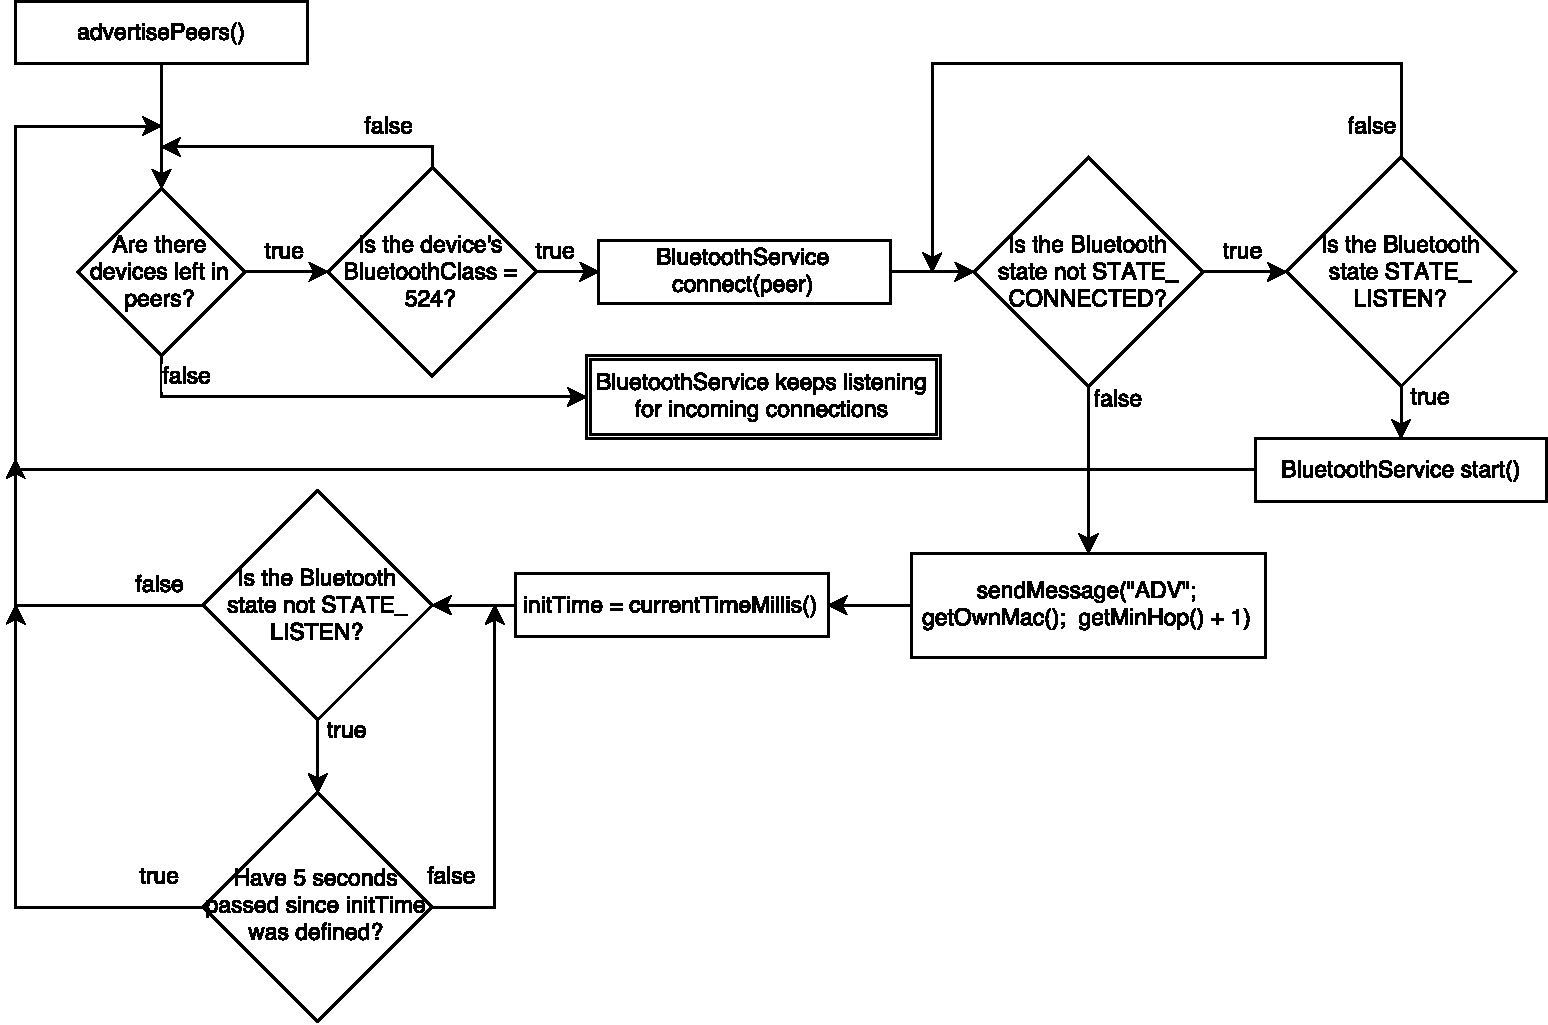
\includegraphics[width=1\textwidth]{images/advertise_flux.pdf}}
	\caption{\label{fig:advflux} Fluxogram of the advertising process from the point of a sender}
\end{figure}

\subsubsection{Receiving an Advertising Message}
\label{subsubsec:rcvadv}

It is now covered how the transmitter of an advertise message operates, however, to fully understand the advertising process it is necessary to analyse the receiver device and how it handles this message.

So, on the receiver device, after the reception of the advertising message, the handler receives the transferred message bytes from the \textit{BluetoothService}. To understand how this is performed the \textit{Handler mHandler} must be explained first.

The method \textit{handleMessage()} is overwritten, in order to control what is done with the received \textit{Message}, see \cite{msgclass} for full documentation on this Android class. There are seven possible \textit{Message} types: \textit{MESSAGE\_STATE\_CHANGE} used to notify of a Bluetooth state change, \textit{MESSAGE\_WRITE} received when this device has sent a message, \textit{MESSAGE\_READ} to notify that this device has just received a message, \textit{MESSAGE\_DEVICE\_NAME} received when there is a new connection, gives the name of the connected device, \textit{MESSAGE\_TOAST} for when the user needs to be notified on something regarding the \textit{BluetoothService}, \textit{FILE\_READ} to notify of the reception of a web page by the device and \textit{FILE\_WRITE} for debug purposes, received when this device sends a web page.

For the receiver's advertising process the focus will be on the \textit{MESSAGE\_READ} \textit{Message} type. If the \textit{Message} is identified as a \textit{MESSAGE\_READ} the \textit{Handler} will construct a \textit{String} from the received bytes. From this \textit{String}, the device is now able to extract what type of message it is, \textit{i.e.}, an \textit{ADV}, a \textit{RQT}, a \textit{RSP} or a \textit{FAIL}. In case the message is not a response the \textit{BluetoothService} is restarted and will listen to incoming connections. However, if the message is a response, the service is not restarted, this will be analysed in the next subsection.

After the message is converted to a \textit{String}, it is passed to the method \textit{analyzeMessage()}, where the device will see how to deal with the received message. Here, the message type is assessed, in this case the focus will be the \textit{ADV} type. If the message is identified as an advertising message the method will extract its estimate and compare it to the device's best estimate, retrieved from \textit{getMinHop()}. If the comparison concludes the received estimate does not top the previous best, the routing table is updated with the received estimate and \gls{MAC} address, through \textit{updateRouteTable()}, previously explained. Otherwise, it means the device has found a better way to reach the Internet, so after the routing table is updated, the variable \textit{discoveryFinished} is set to false and the discovery process is done again, through the method \textit{doDiscovery()}.

\begin{figure}[ht]
   \noindent\makebox[\textwidth]
    {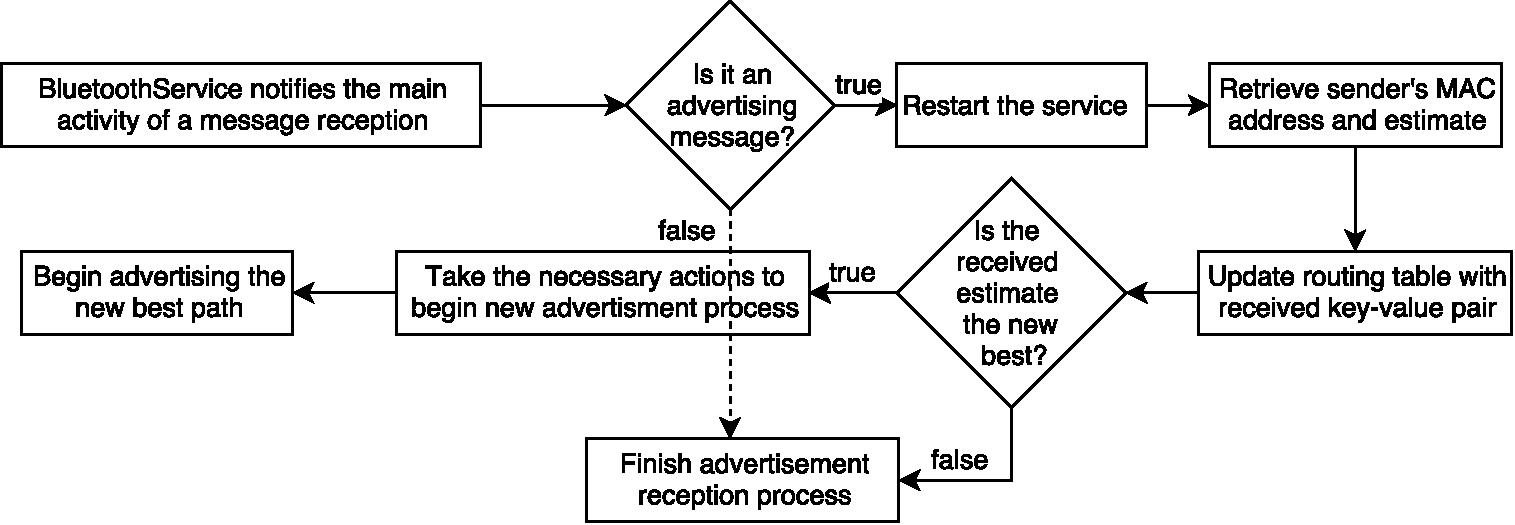
\includegraphics[width=1\textwidth]{images/recv_advertise_flux.pdf}}
	\caption{\label{fig:recvadvflux} Fluxogram of the advertising process from the point of a receiver}
\end{figure}

In figure \ref{fig:recvadvflux} it is shown a fluxogram for a receiver device and its order of instructions. The device ends this process either with a \textit{doDiscovery()} method call or by "listening" to incoming connections. Some aspects of the fluxogram are simplified as they do not concern this process and will be discussed later.

\begin{figure}[ht]
   \noindent\makebox[\textwidth]
    {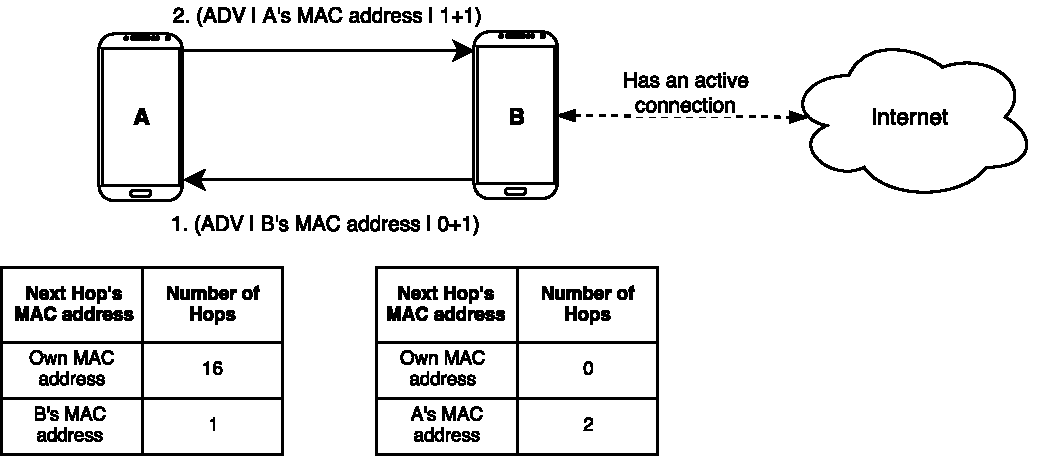
\includegraphics[width=1\textwidth]{images/adv_example_2.pdf}}
	\caption{\label{fig:adveg2} Example 1: State of the two devices after the advertising process is done} 
\end{figure}

To summarize, in figure \ref{fig:adveg2} the example with devices A and B from figure \ref{fig:adveg1} is extended. Now device B has advertised to its peers, which include device A. Upon receiving this message, device A proceeded to store the information in its routing table, followed by and advertise from itself, since the new estimate tops the previous one. After this is concluded both devices have the shown routing tables, and A knows it routes to B, while B routes to itself, since A provides a poorer estimate.

If A advertises first the result would be the same, since when B is advertising A would still receive a better estimate and would advertise again. When B receives the second advertise from A it will overwrite the previous entry, maintaining the same values.

Now it should be clear how the discovery and advertising process is performed and what is the code executed at each time of the process. This is the basis of the next subsection, since without it the devices would not be able to reach the Internet unless they already had the connection.

By giving each device a full view of its vicinity it is possible to establish a network in which every device knows the best path instantly. This is done by what was described above, from discovery to advertisement. The next subsection will refer to the next step, where the devices already have their routing tables populated and are ready to exchange web pages. 

\subsection{Exchange of Web Pages}

In this subsection the logic created and implemented to exchange the web pages will be explained, in detail, also an example, similar to the previous one will be shown to better demonstrate the processes. This analysis will be mainly focused in appendix \ref{appendix:BtActivity}. However, before that it is necessary to explain the routing table related to the exchange of web pages, previously mentioned in subsection \ref{subsec:disandadv} and referred to as response table.

The main purpose of this table is to provide a destination for a response message. Once a device has received a request and it has an Internet connection, it should know where to send back the response. This would be easy if only this case applied, it would simply send back the response from where it received the request. But, in the case this device is a "bridge" node, \textit{i.e.}, it is simply a node that forwarded a request, it may have received requests from different devices and it still needs to be able to differentiate each message and decide which device to send back the response to.

The response table has a similar structure to the routing table, see figure \ref{tab:rspTables}, but it serves a different purpose. Similarly to routing table, the response table is defined in \textit{RoutingApp} class, it is an object of the Java class \textit{Map}.

\begin{table}[ht]
\centering
\bgroup
\def\arraystretch{2.5}
\begin{tabular}{|c|c|}
\hline
\textbf{Message ID} & \textbf{Next hop's MAC} \\ \hline
Message ID \#1 & Device X's MAC \\ \hline
Message ID \#2 & Device Y's MAC \\ \hline
Message ID \#3 & Device Z's MAC \\ \hline
... & ... \\ \hline
Message ID \#9 & Device X's MAC \\ \hline
\end{tabular}
\egroup
\caption{Response table example and format}
\label{tab:rspTables}
\end{table}

Despite the similarities, there is one difference between the two: routing table maps \textit{Strings} to integers whereas response table maps integers to \textit{Strings}. The latter is used to associate message identifiers, the integers, with the \gls{MAC} address of the next destination of a response, the \textit{String}.

The table is defined as \textit{rspTable} and it has two associated methods: \textit{updateRspTable()} and \textit{getRspHop()}. The first method is used to add new rows to the response table, it is similar to routing table's method \textit{updateRouteTable()}, and makes use of the same Java method \textit{put()}, previously explained. Although it has a slight difference in logic, since this method will not update rows, it will always insert new rows, seeing the message identifiers are unique there should be no duplicate entries.

The second method, \textit{getRspHop()} is used to retrieve the \gls{MAC} address associated to a certain message identifier, that is as a parameter. In case a table entry is found for that specific identifier, the associated \gls{MAC} address is returned, otherwise it will return null, notifying the application that no entry was found and thus, the response will not be routed.

For the example three devices are used: A, B and C. Where device C has an active Internet connection, as seen in figure \ref{fig:example1.0}. In this figure it is possible to see the routing tables of each device after this process is completed. Device A will choose B to send a request and B will choose C, since they provide the best estimates, respectively.

\begin{figure}[ht]
   \noindent\makebox[\textwidth]
    {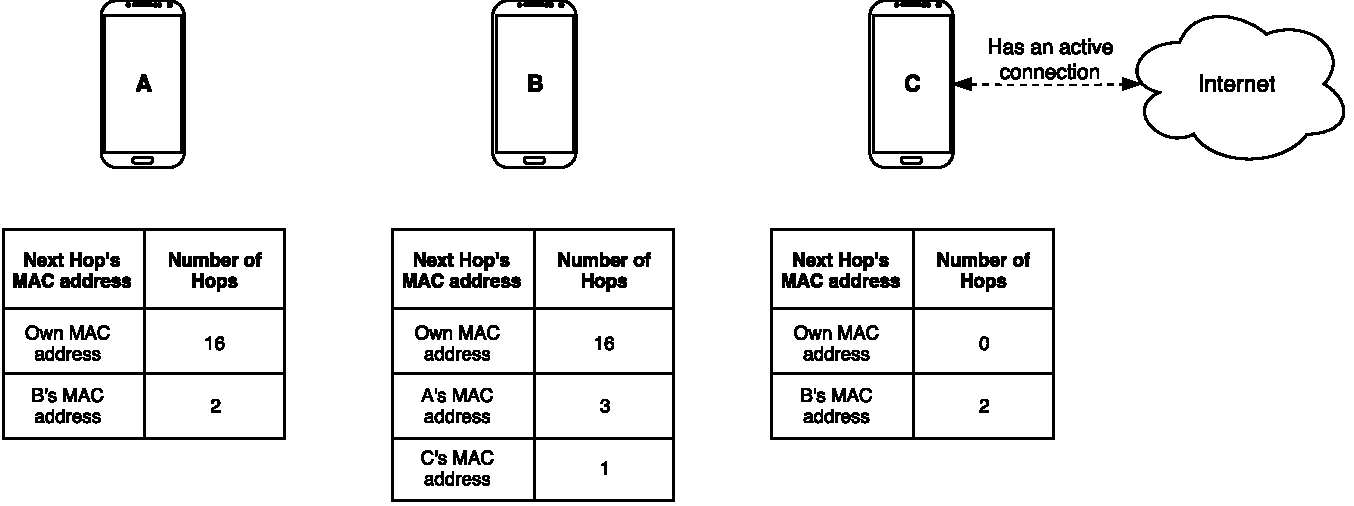
\includegraphics[width=1\textwidth]{images/example_1_0.pdf}}
	\caption{\label{fig:example1.0} Example 2: State of the routing tables of the three devices}
\end{figure}

\subsubsection{Sending a Request Message}
\label{subsubsec:sendrqt}

Now that the logic and implementation behind the response table is understood it is possible to start explaining the actual process of web page exchanging. Starting by the definition of variables, in \textit{BtActivity} class, it can be divided into three sections: the first being the definition of variables that will identify the different elements seen by the user, a \textit{Button}, to submit requests, an \textit{EditText}, for the user to input the requested \gls{URL} and a \textit{WebView}, to manage the actions related to web pages.

It is then possible to see the definition of the constants relative to the \textit{BluetoothService} class, see \ref{subsec:btconn}. The possible \textit{Message} types received from the service are defined: \textit{MESSAGE\_STATE\_CHANGE}, \textit{MESSAGE\_READ}, \textit{MESSAGE\_WRITE}, \textit{MESSAGE\_DEVICE\_NAME}, \textit{MESSAGE\_TOAST}, \textit{FILE\_READ} and \textit{FILE\_WRITE}. These types are explained in \ref{subsubsec:rcvadv}, and \textit{MESSAGE\_READ} was already mentioned, although only covering the advertising messages.

Finally, the last block of variables, containing various definitions relative to this class. \textit{msgID} is the variable that concerns this process of exchange, it stores the message identifier of the last received request or response.

\begin{figure}[ht]
   \noindent\makebox[\textwidth]
    {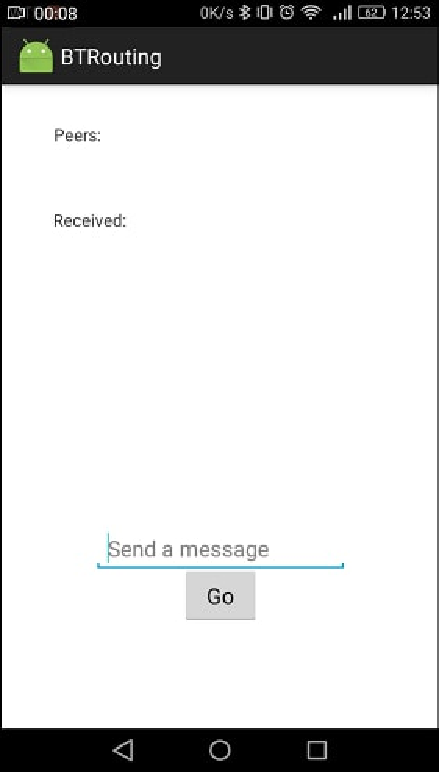
\includegraphics[width=0.3\textwidth]{images/initScreen.pdf}}
	\caption{\label{fig:initScreen} User interface for the sending of request messages}
\end{figure}

In figure \ref{fig:initScreen} it can be seen the display of the main activity page, it has five main elements: a place where the \textit{peers} list will be displayed, at the top. The received messages, this is optional and used for debugging as it would incur in severe security issues, so it should be removed if not for debugging. An \textit{EditText}, see \cite{edittext} for documentation on this Android feature, used to allow the user to input the web page he/she desires and to capture this input to be processed. A \textit{Button}, to notify the activity it should now begin the process of requesting the web page. Finally, a \textit{WebView}, see \cite{webview} for documentation on this feature, that is hidden from user view and will remain so until the user receives the response to its request.

Assuming the device already established the best route to reach the Internet, the journey of the request, from the user input to the display of the response, will be explained. Starting by the user input, has said above, a \textit{Button} and an \textit{EditView} are defined, so a user interface is created, in order to send requests based on the user input. This is defined in method \textit{onStart()}, from appendix \ref{appendix:BtActivity}, after the routing table is first populated and the discovery is started, discussed in \ref{subsec:disandadv}. The variables previously defined, \textit{goButton} and \textit{mEdit} are matched to the elements in figure \ref{fig:initScreen}, so they can be identified by the application.

The \textit{Button} class' method \textit{onClick()} is then overwritten, meaning it is tailored for the specific needs of this application. This method has the purpose of responding to a click of the user in the specific button, to this click the method must associate an intent to send a request message. With these parameters the method \textit{onClick()} is set to call \textit{sendRequest()}.

The \textit{sendRequest()} method receives as parameters: a boolean to identify if the intent is coming from the owner of the request or from a mediator node, an integer that corresponds to the message identifier and a \textit{String} containing the requested \gls{URL}.

Since this particular request comes directly from the user input, this method is initially called by this device with the following arguments: "true", "-1" and the user input text. The "true" value is used whenever the device is the one issuing the request, \textit{i.e.}, whenever it is its origin. "-1" is used when the value of the message identifier is not important, in this case, since this device is the "owner" of the request, a random message identifier will be generated. Finally, to identify the web page requested, the user input \gls{URL} is passed.

\begin{figure}[ht]
   \noindent\makebox[\textwidth]
    {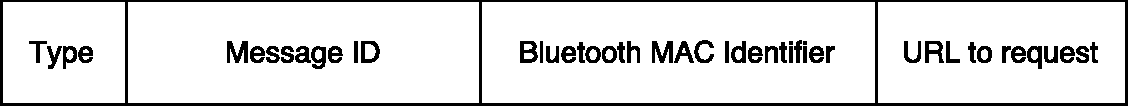
\includegraphics[width=0.9\textwidth]{images/rqtmessage.pdf}}
	\caption{\label{fig:rqtmsg} Request message format}
\end{figure}

In figure \ref{fig:rqtmsg} a generic request message is shown. Its format does not differ much from the one presented in figure \ref{fig:advmsg}, however there is a new field, the \textit{Message ID}, a unique identifier representing each message that will be useful to keep track of what is each message's payload and sender. The \textit{\gls{URL} to request} is the web page's \gls{URL} the user is trying to access, it is considered to be the payload of the message.

Continuing the analysis on method \textit{sendRequest()}, the first thing that is done is to retrieve the next hop, to whom the device shall send its request, this is done by calling the method \textit{getNextHop()}, defined in \ref{appendix:RoutingApp}. This method returns the \gls{MAC} address of the device's peer who provides the best path. \textit{getMinHop()} is called to retrieve the best estimate, to which is applied the function \textit{getKeyFromValue()}, alongside with the routing table, see subsection \ref{subsubsec:disc} to get more a detailed explanation on how these two methods work. This combination should return the desired \gls{MAC} address, however if the best estimate is 16, "null" is returned to notify the device that no path was found.

Once the \gls{MAC} address of the next hop is attained, \textit{sendRequest()} compares it with "null", to ensure there is an actual device to connect to. In case this comparison is successful, meaning there is no next hop, the method \textit{sendFail()} is called. Since this device is the owner of the request, the \textit{sendFail()} method will not send a failure notification to another device, it will simply notify the user of the failure. The method \textit{sendFail()} will be discussed further on this subsection.

In the case of the device having a valid next hop, the connection is performed, similarly to the advertising connections, by the \textit{BluetoothService connect()} method. The first cycle described in the advertising process is now repeated here, to ensure the connection is established before sending the message, with the single difference of in case of failure, \textit{i.e.}, the Bluetooth state becoming \textit{STATE\_LISTEN}, \textit{sendFail()} is called again, to notify possible predecessors of this request, however in this case it does not apply.

If the cycle is finished and everything is completed without any incidents, the method verifies the first argument, the boolean variable to identify if the device is the owner of the request. If the device is the owner a random message identifier is generated through the Java class \textit{Random}, see \cite{random}. Once the identifier is generated, the message is sent with the parameters: "RQT" as \textit{Type}, the value of the generated random as \textit{Message ID}, the device's \gls{MAC} address gotten through \textit{getOwnMAC()} as \textit{Bluetooth MAC Identifier} and the received \gls{URL} from the arguments as the \textit{\gls{URL} to request}, as seen in figure \ref{fig:rqtmsg}. The response table is also updated with the newly generated message identifier and device's \gls{MAC} address, through \textit{updateRspTable()}.

Otherwise, if the device is not deemed as the owner, there is no random identifier generation, since the value will come from the received request. Also the response table is not updated, since it will be updated earlier in the receiving process, that will be the next focus. However, the message is sent as before, with the slight difference that the \textit{Message ID} is now the one received as an argument.

\begin{figure}[ht]
   \noindent\makebox[\textwidth]
    {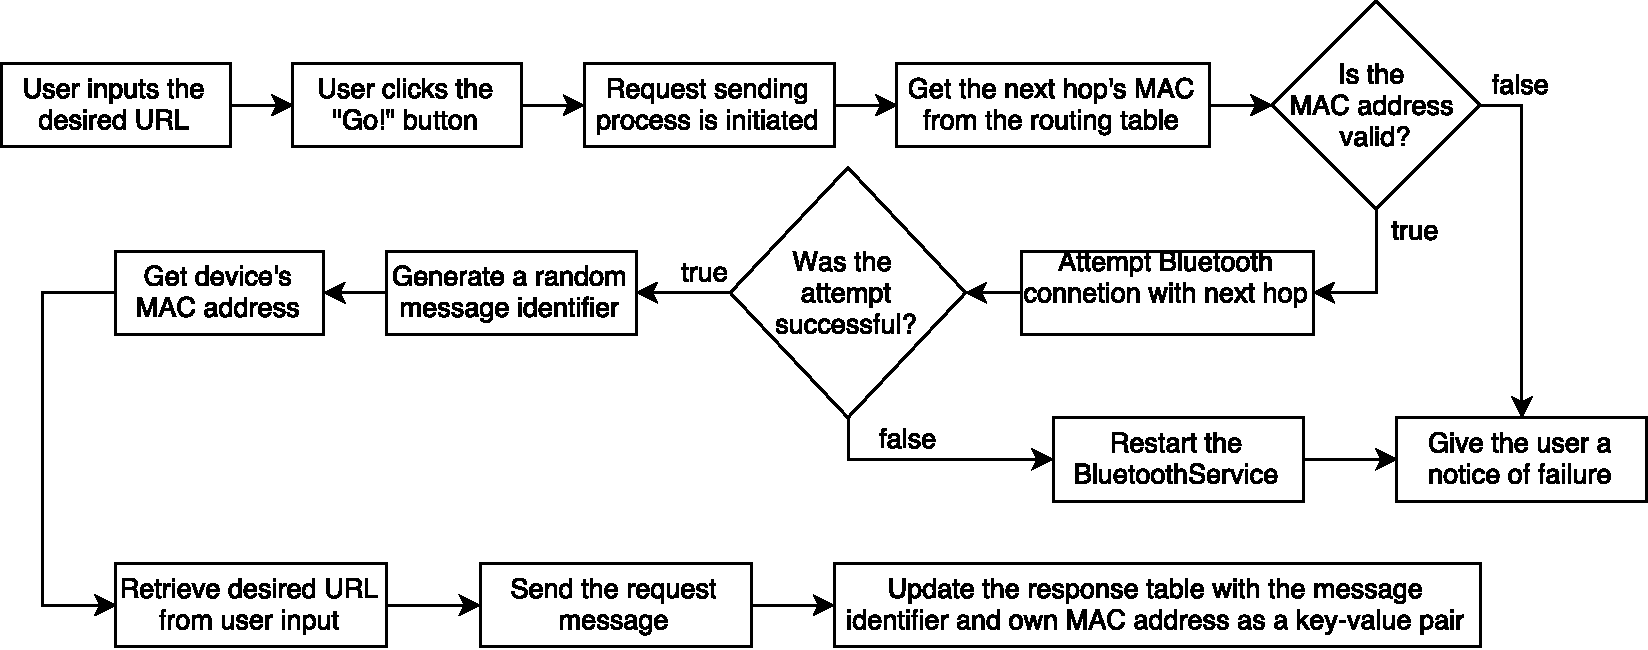
\includegraphics[width=1\textwidth]{images/rqtflux.pdf}}
	\caption{\label{fig:rqtflux} Fluxogram of the request sending process}
\end{figure}

In figure \ref{fig:rqtflux} a fluxogram representing the process of sending request message is presented. It provides a better overview of the code hierarchy, and when is each method called. Once the process is finished the device keeps listening to incoming connections, changing the Bluetooth state to \textit{STATE\_LISTEN}.

\subsubsection{Receiving a Request Message}
\label{subsubsec:rcvrqt}

The request receiving process is similar to the advertise, the receiver connects to the sender and receives the bytes from the request sent. As before, the bytes are transmitted from the \textit{BluetoothService} to the main activity, through a \textit{MESSAGE\_READ Message} and the \textit{mHandler} receives them. After comparing the received \textit{Message} to the possible types, explained in subsection \ref{subsubsec:rcvadv}, and concluding it is a \textit{MESSAGE\_READ} the \textit{Handler} converts them to a \textit{String}. Since the newly created \textit{String} is not a response, the \textit{BluetoothService} is restarted and \textit{analyzeMessage()} is called taking as argument the \textit{String}.

In \textit{analyzeMessage()} the argument \textit{String} is compared to the possible message types, \textit{ADV}, \textit{RQT}, \textit{RSP} and \textit{FAIL}. It will now be identified as a response, due to the analysis of the message type, see figure \ref{fig:rqtmsg}, and immediately the message identifier is saved in the variable \textit{msgID}.

In the request sending process it was mentioned that, in case the device was not the owner of request, it would not update the response table. This was due to the fact that, for the devices that are not the owners of the request, this process is done here, in \textit{analyzeMessage()}. So, the routing table is updated with the message identifier and \gls{MAC} address of the sender, retrieved from the message.

Two different approaches can now be taken: one regards the devices with Internet connection and the other the devices without one. To define which approach is taken by the device a quick check of the Internet connection status is performed, via the method \textit{getHasNet()}. If the result is false, meaning the device has no Internet connection, the request will be forwarded to the next hop to reach a device with Internet. To do this, the device calls \textit{sendRequest()} with arguments: false, the message identifier, retrieved from the received message and the \gls{URL} requested, also retrieved from the message. The method follows the same steps as before, described in \ref{subsubsec:sendrqt}.

If the result of the \textit{getHasNet()} query returns true, it means the device has an Internet connection and, as such, it is a final destination. This means the device will now be the communication link with the Internet and it needs to retrieve the requested web page and send it backwards until it reaches the owner of the request. This process begins by calling the method \textit{getPage()}, that receives the requested \gls{URL} and the message identifier, both retrieved from the received message.

In \textit{getPage()} the web page is downloaded via the \textit{WebView}, mentioned in \ref{subsubsec:sendrqt}. A new \textit{WebViewClient} is created, see \cite{webview} for documentation on \textit{WebView} and its features, such as the \textit{WebViewClient}. This client is different from the usual, since the device does not want to display the downloaded page.

The methodology to save the web page had several possibilities, such as saving the web page as an image, saving only the \textit{HTML} content or saving each element of the page individually. The first two methods are not complete, meaning the web page could lose some of its features, \textit{e.g.} dynamic images, search fields, \textit{etc.}. The third method would fully download the web page, however it would require additional logic to save the different elements in the same directory and to arrange them to re-create the web page with its initial format.

The method \textit{saveWebArchive()} provides a complete solution to this problem, it is a method specific to the \textit{WebViewClient}'s class, see \cite{webview} and it solves the problem of third method, since it downloads each element but compiles them in a web archive, that can be decompressed easily by \textit{WebView}. Thus, it proved to be the better solution for this problem.

To implement this methodology, the method \textit{onPageFinished()}, from \textit{WebViewClient}'s class, is overwritten. This method is used to do something after the web page is finished loading. So, a new \textit{File} is created in the application's directory, with the name "file.mht". If the file creation succeeds, the web page is downloaded and saved in the created file, via \textit{saveWebArchive()}. In order to guarantee the web page is downloaded and saved before the response is set, a \textit{waitForWebPage} downloader is created and executed.

The \textit{waitForWebPage} class can be seen in appendix \ref{appendix:BtActivity} and was created with the sole purpose of guaranteeing the web page transfer is completed before the response is sent. If this check is not performed, it is possible that, for large web pages, the response file will be incomplete and thus not displaying correctly the requested \gls{URL}.

It extends an \textit{AsyncTask}, used to perform background operations and send the results to the main thread, see \cite{async} for the full documentation. It starts by creating a variable \textit{file} that will contain the address where the web page will be saved. The method \textit{doInBackground()} is overwritten, as it always has to be in an \textit{AsyncTask}, since it contains what operations to be performed.

In this method it is continuously checked if the variable \textit{file} has a size bigger than 0 bytes. Whenever this condition is verified, it means the web page was saved successfully. The \textit{onPostExecute()} method, used to send the results to the main thread, is also overwritten and, once this thread reaches this point, it means the device is ready to send the response, so \textit{sendResponse()} is called.

\begin{figure}[ht]
   \noindent\makebox[\textwidth]
    {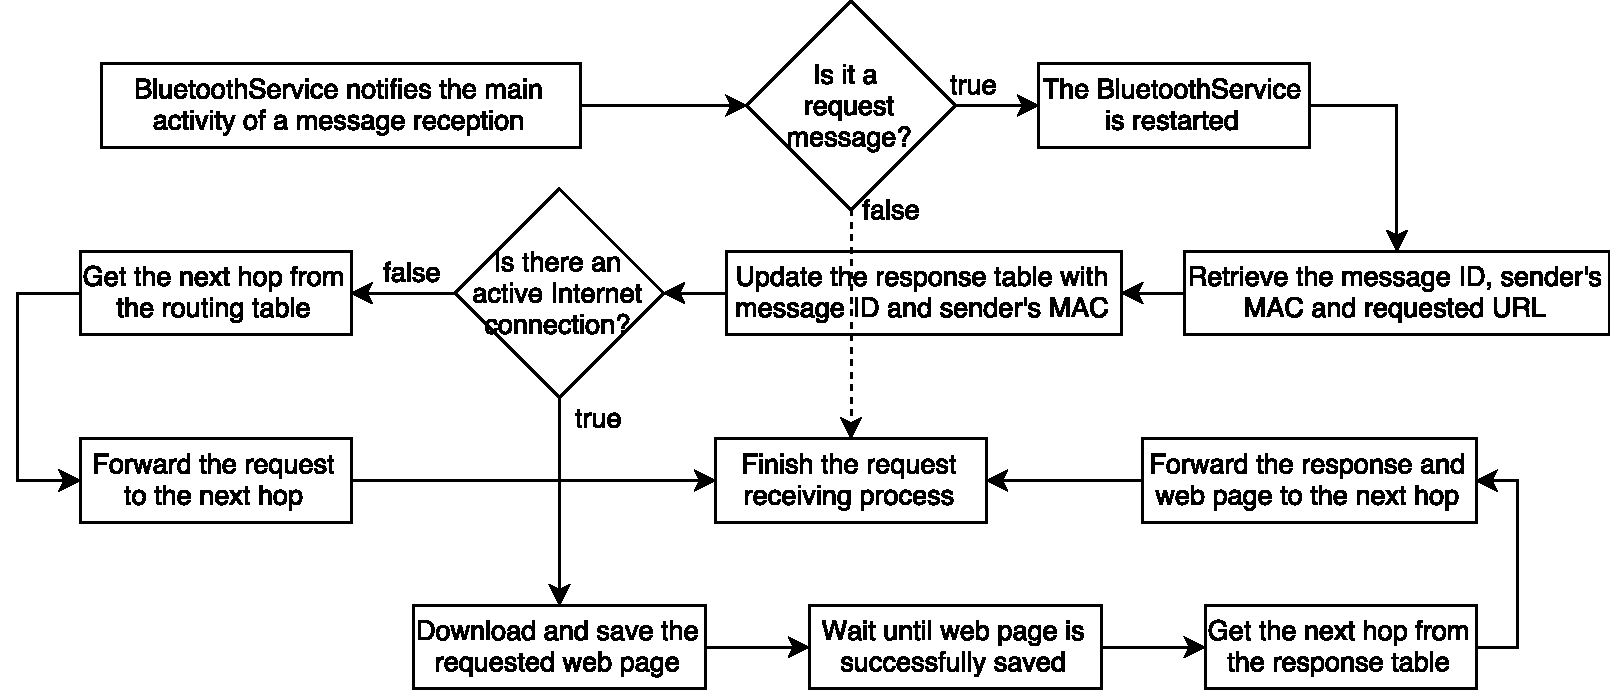
\includegraphics[width=1\textwidth]{images/rqt_rcv_flux.pdf}}
	\caption{\label{fig:rqtrcvflux} Fluxogram of the request receiving process}
\end{figure}

In figure \ref{fig:rqtrcvflux} it is possible to see a fluxogram of this process. The process, as shown in the figure, ends either with sending a new response or a new request, depending on whether the device has Internet connection or not, respectively.

\begin{figure}[ht]
   \noindent\makebox[\textwidth]
    {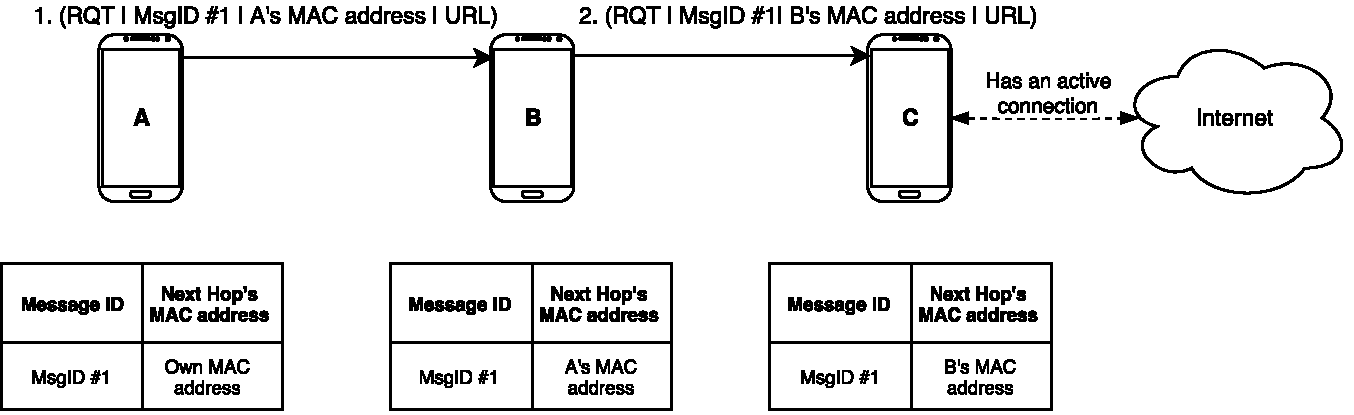
\includegraphics[width=1\textwidth]{images/example_1_1.pdf}}
	\caption{\label{fig:example1.1} Example 2: Request sending and receiving process}
\end{figure}

Resuming the example in figure \ref{fig:example1.0} and supposing the user from device A wants to request a \gls{URL} and inputs it correctly, the device will follow the steps explained in subsection \ref{subsubsec:sendrqt} and check the routing table to establish the next hop. Also its response table will be filled during this action, since it is the owner of the request.

Once that process is completed and the message reaches device B it will update its routing table with the newly received request. After that it checks its own routing table and assesses if it should forward the request or download the page. Since the device does not have an active connection the first option will chosen and the request forwarded to C.

Finally, upon receiving the request, device C will update its own response table with the received message identifier and B's \gls{MAC} address. Having an Internet connection the device will download the web page.

In figure \ref{fig:example1.1} it is shown the above described, as well as the three response tables from the devices once the requests are all sent and the web page downloaded.

\subsubsection{Sending a Response Message and Web Page}
\label{subsubsec:sendrsp}

Once the web page is successfully saved in the device it is possible to send the response back until the owner of the request receives the requested web page. As seen before, \textit{sendResponse()} is called in \textit{onPostExecute()} and it is used to send a response to the next device.

It receives as parameter the message identifier, so that the \gls{MAC} address of the next device can be retrieved from the response table. Thus, having the message identifier and through the method \textit{getRspHop()}, the device retrieves the next hop's \gls{MAC} address. Should the result of this call be null, the response will not be sent. If the result returns a valid \gls{MAC} address, the connection process is performed, along with the cycle to ensure the connection is successful, described in subsection \ref{subsubsec:sendadv}.

\begin{figure}[ht]
   \noindent\makebox[\textwidth]
    {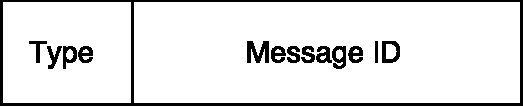
\includegraphics[width=0.4\textwidth]{images/rspmessage.pdf}}
	\caption{\label{fig:rspmsg} Format of a response message}
\end{figure}

Finally, if all the above goes as planned and succeeds, the response is sent with the format seen in figure \ref{fig:rspmsg}, with "RSP" as \textit{Type} and the received argument \textit{msgID} as \textit{Message ID}.

The next step is to send the actual web page to the next hop, but first the sender needs to ensure the response was correctly sent. This is done by the \textit{Handler}, explained in subsection \ref{subsubsec:sendadv}. The \textit{Message} type \textit{MESSAGE\_WRITE} is used for this, since it returns the bytes sent from the device and convert them to a \textit{String}. If the converted \textit{String} is a response message the application concludes the process is completed correctly and proceeds to call the method \textit{sendFile()}.

The \textit{sendFile()} method is called when the device is ready to sent the web page bytes to the next hop. It begins by creating a variable \textit{file}, pointing to the file in the application storage that contains the web page. The size of that file is retrieved through \textit{file.length()} and an array of bytes is created with that same size. This array of bytes will be the place where the web page will be transferred, from the internal storage to the application.

In order to transfer the web page from the file, in the internal storage, to the application a \textit{BufferedInputStream} is used, see \cite{bis} for more documentation on this class. This \textit{BufferedInputStream} instance takes the bytes from the variable \textit{file}, previously described and saves them in the array of bytes, it is then closed to avoid memory leaks.

Once the bytes are transferred to the application the device needs to send them to the next hop, since the connection is still opened, for reasons that will be explained in the next subsection, it is possible to send the bytes without the logic to connect to the next hop. The method \textit{writeFile()} from \textit{BluetoothService} is called and the file bytes is transferred to the next hop as described in subsection \ref{subsubsec:connected}.

The method gets the number of bytes to be sent and divides that size by 990 bytes, getting the number of chunks that need to be sent to the next hop. It then proceeds to send each chunk with a length of 990 bytes, until it reaches the last chunk, sending the remaining bytes.

\begin{figure}[ht]
   \noindent\makebox[\textwidth]
    {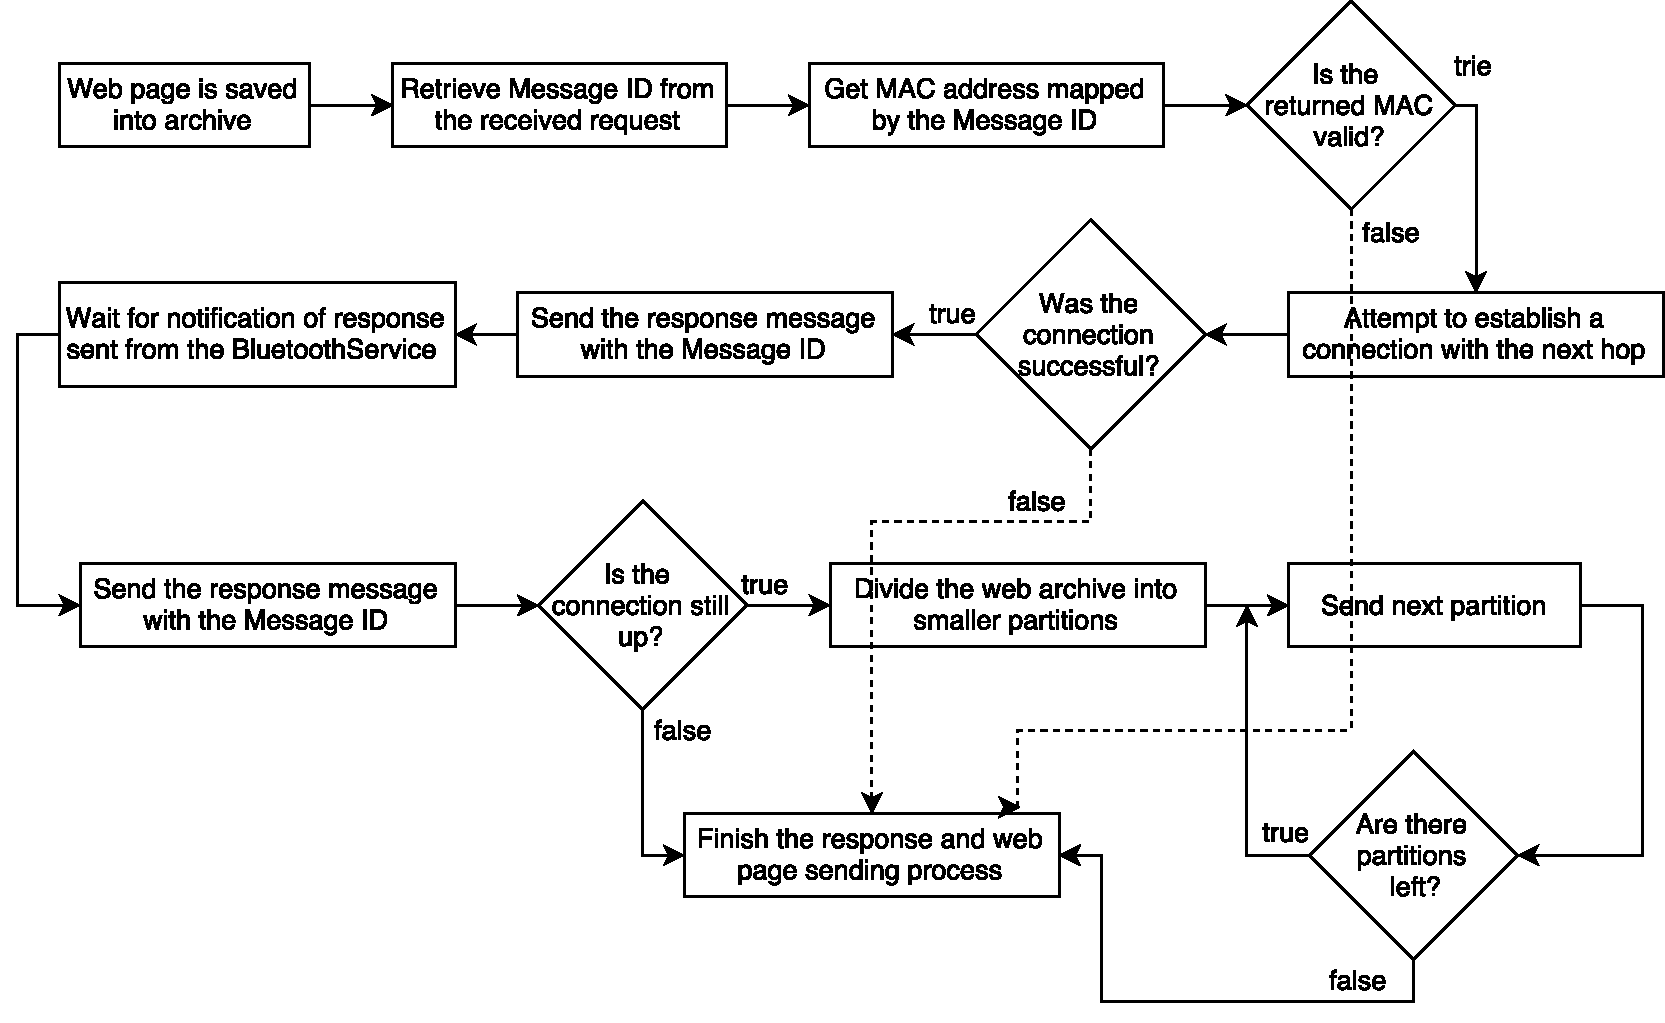
\includegraphics[width=1\textwidth]{images/send_rsp_flux.pdf}}
	\caption{\label{fig:rspsendflux} Fluxogram of the response and web page sending process}
\end{figure}

In figure \ref{fig:rspsendflux} a fluxogram of the response sending response is presented. It shows the process from the saving of the web page to the sending of the same. As previously described the fluxogram ends by dropping the message if there is no valid next hop for that message identifier, by restarting the \textit{BluetoothService} if the connection fails, or by sending the full web page as expected.

\subsubsection{Receiving a Response Message and Web Page}
\label{subsubsec:rcvrsp}

In the receiver side, the web page and response are received and the device must assess if it is the final destination or if it is a relay node for a different device, in which case the web page will not be displayed, but the response and web page are forwarded.

This process begins in the \textit{Handler}, where the notification is notified that a message as been received by a \textit{MESSAGE\_READ}. The received message is compared with the possible types and, since it is a response message, it is identified as such. In the case of a response, the \textit{BluetoothService} is not restarted, since the device benefit from keeping the connection active to avoid further delays in re-connecting to receive the web page, also mentioned in subsection \ref{subsubsec:sendrsp}. Instead, the \textit{BluetoothService}'s variable \textit{fileReady} is set to "true", meaning the device is has received a response message and is ready to receive the associated web page.

The message is then sent to method \textit{analyzeMessage} as a \textit{String}, where the message identifier will be saved to \textit{msgID}, retrieved from the response message, see figure \ref{fig:rspmsg}. Having the message identifier the method compares the device's \gls{MAC} address to the one returned from \textit{getRspHop()} for that same message identifier. If both addresses match the device is the destination and the owner of the request, so the web page will be displayed. Otherwise, the response will be forwarded to the next destination.

The sender will then proceed to transfer the web page bytes from one device to another. At this point the receiver is expecting a file, since the variable \textit{fileReady} is set to "true". This shifts the \textit{BluetoothService} reception logic from receiving a \textit{String} to receiving a web page, see subsection \ref{subsubsec:connected} for more details on this logic.

A variable \textit{output} is created, where each 990 bytes chunk is saved. When the transfer reaches the last chunk, identified by its size, which will be smaller than 990 bytes, the information contained in this variable is passed to a byte array, that will be sent back to main activity via a \textit{FILE\_READ Message}.

Once the main activity's \textit{Handler} receives this notification it copies the bytes received from \textit{BluetoothService} to a file in the application's directory. The \textit{BluetoothService} is restarted and the variable \textit{fileReady} is set to "false", as the device does not expect to receive anymore files for the time being. A new comparison between the device's own \gls{MAC} and the result of \textit{getRspHop} for that specific message identifier is made. If the result is false, meaning the device is not the destination, the response is forwarded through \textit{sendResponse}, with the corresponding message identifier, see \ref{subsubsec:sendrsp} for information on this process.

However, if the device is deemed the owner of the original request and thus the destination of the web page, the method \textit{loadPage()} is called, were the logic to display the web page is performed. First the \textit{WebView} instance is set to load web pages first from cache instead of directly trying to access the network, via \textit{setCacheMode(WebSettings.LOAD\_CACHE\_ELSE\_NETWORK)}, see \cite{webview} for more documentation. It is followed by setting the \textit{WebView}'s visibility to \textit{VISIBLE}.


There is one important aspect of this application that was not yet discussed. When the requester receives the web page, it might be needed to request multiple pages, for instance in a Google search, the user requests the front page and then inserts its query and a subsequent page is requested. This logic has to be reflected in the application for it to be deemed useful and usable. If the user had to go back and input each \gls{URL} by itself the application would have no real application.

\textit{WebViewClient}'s class may have a solution to this problem. The class method \textit{onReceivedError} is triggered whenever the \textit{WebView} receives an error, meaning it is possible that, whenever a "no Internet" error is received logic can be created in order to prevent the \textit{WebView} to display that error and instead create a request with the \gls{URL} that returned the error.

To do that, this method is overwritten, beginning by loading the page "about:blank", a page composed of a white screen, in order to avoid the user seeing the error page. A request message is then sent, via \textit{sendRequest} with the arguments: "true", -1 and the \gls{URL} that originated the error, see \ref{subsubsec:sendrqt} for a reminder on how this process is carried. Alongside this, a new \textit{WebChromeClient} is assigned, to handle the display of the web page, see \cite{webview} for more information on this class.

Finally, the web page is displayed via the \textit{WebView} method \textit{loadURL}, which for Android versions superior to 5.1 works perfectly. However if the device's Android version is prior to that the archive where the web page is saved has a different formatting and, as such, needs to be compiled again, via \textit{loadArchive()} by calling \textit{WebView}'s method \textit{loadDataWithBaseURL()} with data retrieved from the saved archive with the methods \textit{getStringFromFile()} and \textit{convertStreamToString()}, taken from \cite{stack}.

\begin{figure}[ht]
   \noindent\makebox[\textwidth]
    {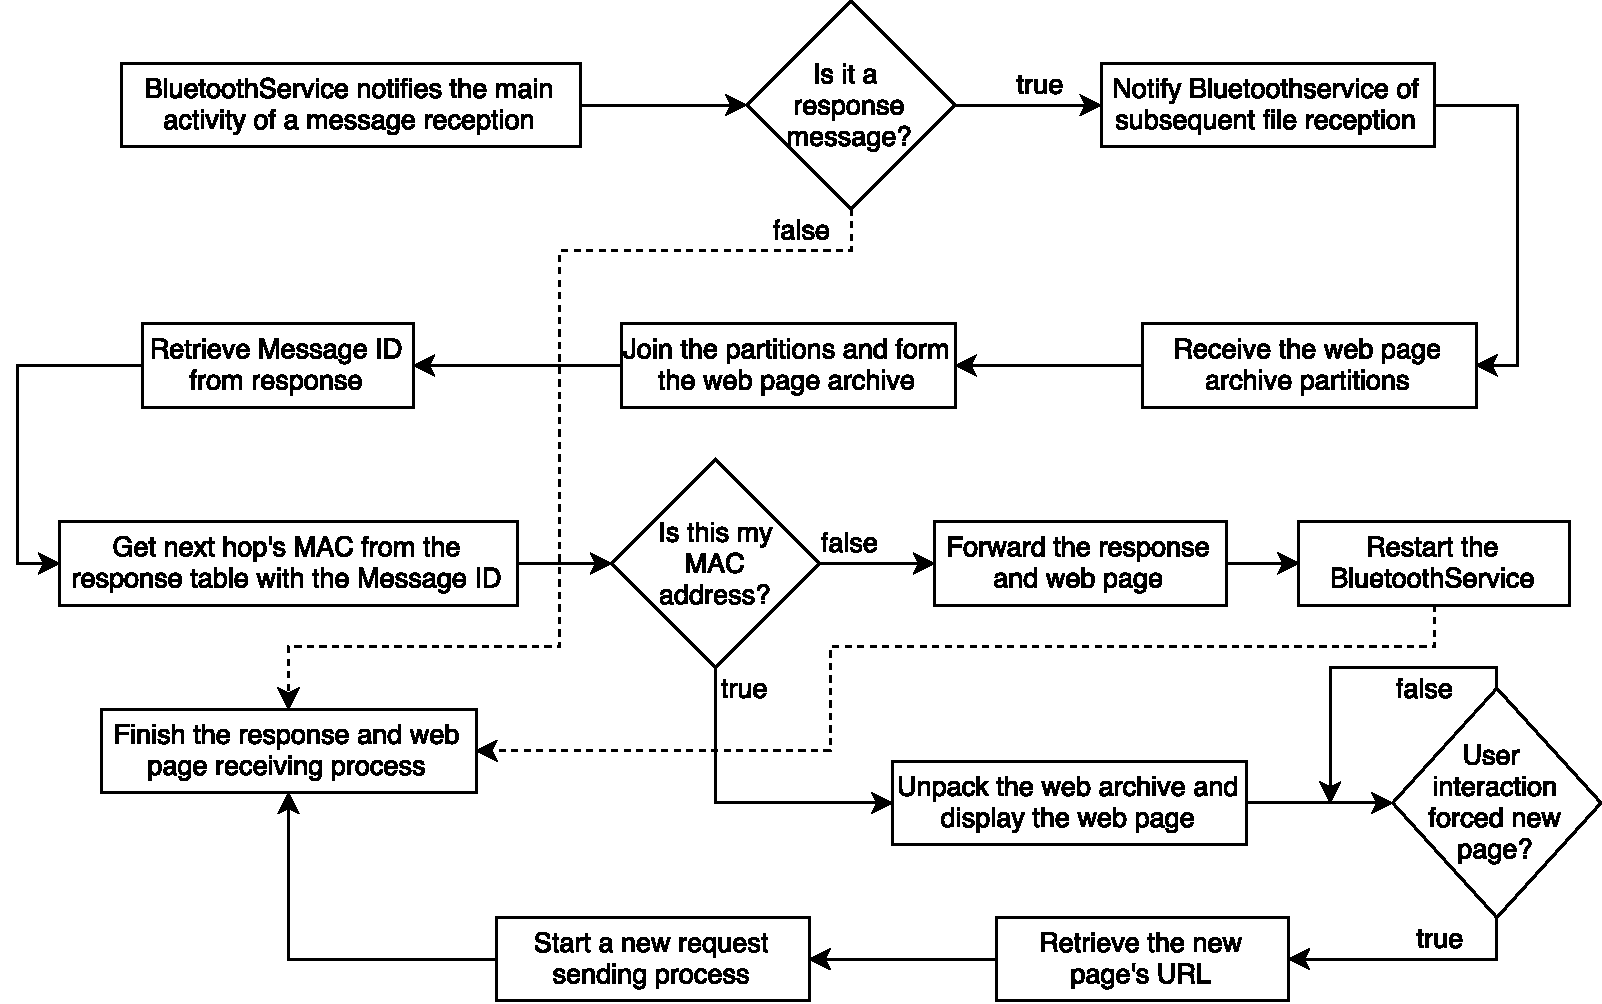
\includegraphics[width=1\textwidth]{images/rcv_rsp_flux.pdf}}
	\caption{\label{fig:rsprcvflux} Fluxogram of the response and web page receiving process}
\end{figure}

In figure \ref{fig:rsprcvflux} a simplified fluxogram of the response and web page receiving process is shown. It is possible to visualize the file receiving logic, as well as the different possibilities for the receiver of the response: forwarding the response or displaying the web page. It is also shown the logic behind the multi web pages request.

With this implementation the user is capable of seeing the request web pages and navigate through those pages without having to manually send each request.

To finalize the example from figures \ref{fig:example1.0} and \ref{fig:example1.1}, device C, after finishing the download of the web page, will check its response table and send a response message to device B, which is the next hop retrieved for that specific message identifier \textit{MsgID \#1}. The response is followed by the web page archive, previously downloaded, as described in subsection \ref{subsubsec:sendrsp}.

Device B receives the response and the web page following the steps previously explained in subsection \ref{subsubsec:rcvrsp} and checks its response table for that message identifier. Device A's \gls{MAC} is returned from that query and that's the destination for B's response, so device B sends the response and web page to A.

A receives the response and web page following the same steps as B. However, when checking the next hop for that message identifier device A gets its own \gls{MAC} address and concludes it is the final destination for that response, proceeding to display the web page requested by the user, as described this subsection.

\begin{figure}[ht]
   \noindent\makebox[\textwidth]
    {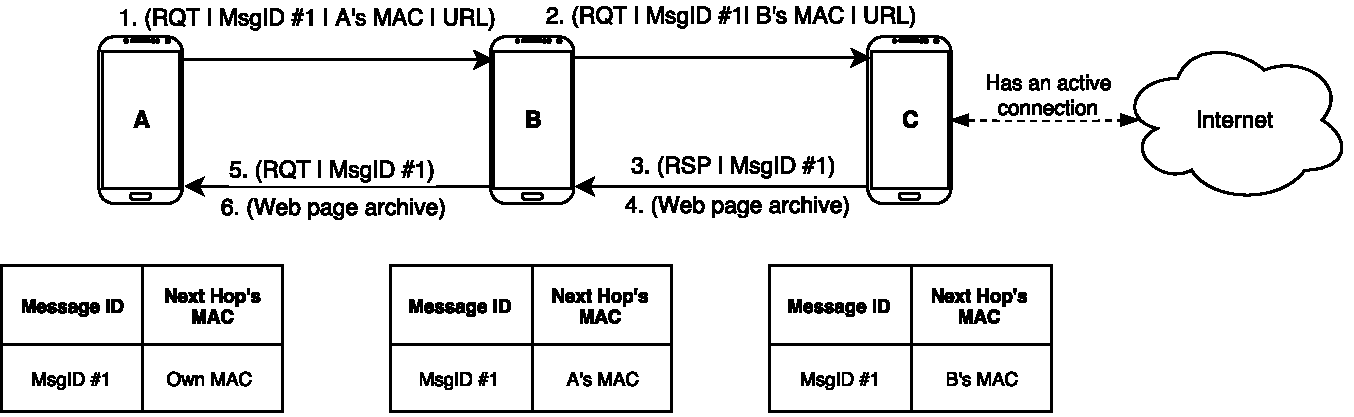
\includegraphics[width=1\textwidth]{images/example_1_2.pdf}}
	\caption{\label{fig:example1.2} Example 2: Sending and receiving of response messages and web pages}
\end{figure}

Figure \ref{fig:example1.2} illustrates this example and messages exchanged between the three devices, as well as the response tables, previously established in figure \ref{fig:example1.1}.











